\documentclass[tikz,border=8pt]{standalone}
% Style commun des schémas : thème clair / sombre (couleurs des thèmes GitHub), fond transparent.
\usepackage[T1]{fontenc}
\usepackage{tgheros}
\renewcommand{\familydefault}{\sfdefault}
\usepackage{tikz}
\usetikzlibrary{positioning,arrows.meta,calc,fit,backgrounds}
\ifdefined\darktheme
  \definecolor{fg}{HTML}{E6EDF3}  \definecolor{muted}{HTML}{9198A1}
  \definecolor{line}{HTML}{8B949E} \definecolor{boxfill}{HTML}{151B23}
  \definecolor{boxline}{HTML}{3D444D}
  \definecolor{blue}{HTML}{4493F8} \definecolor{orange}{HTML}{DB6D28}
  \definecolor{green}{HTML}{3FB950} \definecolor{red}{HTML}{F85149}
  \definecolor{purple}{HTML}{AB7DF8}
\else
  \definecolor{fg}{HTML}{1F2328}  \definecolor{muted}{HTML}{59636E}
  \definecolor{line}{HTML}{59636E} \definecolor{boxfill}{HTML}{F6F8FA}
  \definecolor{boxline}{HTML}{D1D9E0}
  \definecolor{blue}{HTML}{0969DA} \definecolor{orange}{HTML}{BC4C00}
  \definecolor{green}{HTML}{1A7F37} \definecolor{red}{HTML}{CF222E}
  \definecolor{purple}{HTML}{8250DF}
\fi
\tikzset{
  every node/.style={text=fg, font=\small},
  block/.style={draw=boxline, fill=boxfill, rounded corners=3pt, line width=0.7pt,
                minimum height=11mm, minimum width=30mm, align=center, inner sep=5pt},
  sub/.style={font=\scriptsize, text=muted},
  wire/.style={line width=1pt, -{Stealth[length=2.6mm]}},
  biwire/.style={line width=1pt, {Stealth[length=2.6mm]}-{Stealth[length=2.6mm]}},
  lbl/.style={font=\scriptsize, text=muted, fill=none, inner sep=2pt},
}

\begin{document}
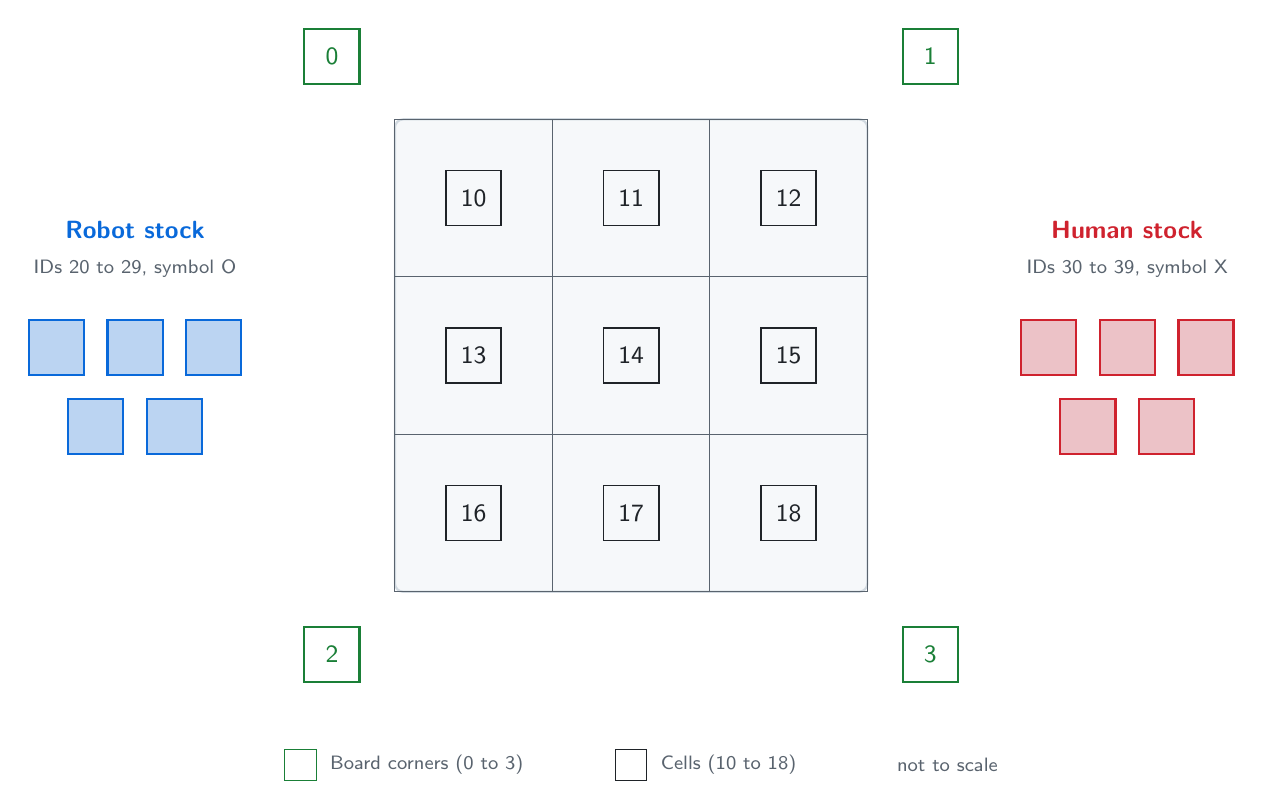
\begin{tikzpicture}[x=10mm,y=10mm]
  % plateau 3x3 : cases 10-18, lecture gauche -> droite, haut -> bas (MAPPING_CASES)
  \draw[boxline, fill=boxfill, rounded corners=3pt, line width=0.8pt] (0,0) rectangle (6,6);
  \foreach \i in {0,...,8}{
    \pgfmathtruncatemacro{\c}{mod(\i,3)} \pgfmathtruncatemacro{\r}{\i/3} \pgfmathtruncatemacro{\id}{10+\i}
    \draw[line, line width=0.4pt] (\c*2,6-\r*2) rectangle ++(2,-2);
    \node[draw=fg, line width=0.6pt, minimum size=7mm, inner sep=0pt, font=\small] at (\c*2+1, 5-\r*2) {\id};
  }
  % coins 0-3
  \foreach \p/\id in {(-0.8,6.8)/0, (6.8,6.8)/1, (-0.8,-0.8)/2, (6.8,-0.8)/3}
    \node[draw=green, text=green, line width=0.8pt, minimum size=7mm, inner sep=0pt, font=\small] at \p {\id};
  % stocks
  \node[font=\small\bfseries, text=blue] at (-3.3,4.6) {Robot stock};
  \node[lbl] at (-3.3,4.1) {IDs 20 to 29, symbol O};
  \foreach \p in {(-4.3,3.1),(-3.3,3.1),(-2.3,3.1),(-3.8,2.1),(-2.8,2.1)}
    \node[draw=blue, fill=blue!25!boxfill, line width=0.8pt, minimum size=7mm] at \p {};
  \node[font=\small\bfseries, text=red] at (9.3,4.6) {Human stock};
  \node[lbl] at (9.3,4.1) {IDs 30 to 39, symbol X};
  \foreach \p in {(8.3,3.1),(9.3,3.1),(10.3,3.1),(8.8,2.1),(9.8,2.1)}
    \node[draw=red, fill=red!25!boxfill, line width=0.8pt, minimum size=7mm] at \p {};
  % légende
  \begin{scope}[shift={(-1.2,-2.2)}]
    \node[draw=green, minimum size=4mm, inner sep=0pt] at (0,0) {}; \node[lbl, anchor=west] at (0.3,0) {Board corners (0 to 3)};
    \node[draw=fg, minimum size=4mm, inner sep=0pt] at (4.2,0) {}; \node[lbl, anchor=west] at (4.5,0) {Cells (10 to 18)};
    \node[lbl, anchor=west] at (7.5,0) {not to scale};
  \end{scope}
\end{tikzpicture}
\end{document}
